\documentclass{standalone}
\usepackage{tikz}
\usepackage{pgfplots}
\pgfplotsset{compat=newest}

\begin{document}
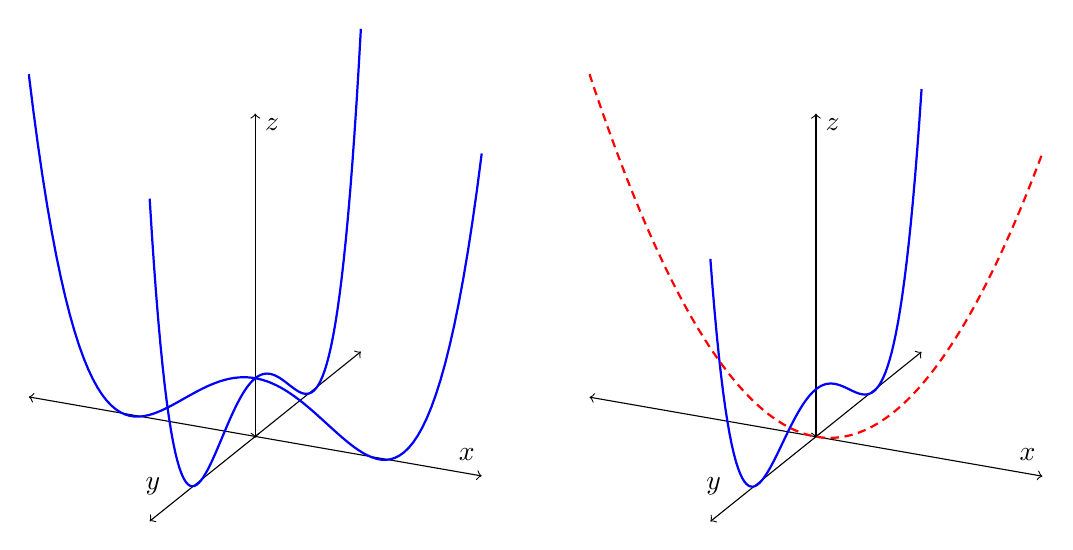
\begin{tikzpicture}
\begin{axis}[view={115}{30},axis lines=middle, name=one, scale only axis, xtick=\empty, ytick=\empty, ztick=\empty, axis line style={<->},xlabel=$y$,ylabel=$x$,zlabel=$z$]
\addplot3[blue,thick,samples=100,samples y=0]({x},{0},{-15*x^2 + x^4 + 55});
\addplot3[blue,thick,samples=100,samples y=0]({0},{x},{-15*x^2 + x^4 + 55});
\end{axis}
\begin{axis}[view={115}{30},axis lines=middle, scale only axis, name=two, at=(one.right of south east), xtick=\empty, ytick=\empty, ztick=\empty, axis line style={<->},xlabel=$y$,ylabel=$x$,zlabel=$z$]
\addplot3[blue,thick,samples=100,samples y=0]({x},{0},{-15*x^2 + x^4 + 55});
\addplot3[red,densely dashed,thick,samples=100,samples y=0]({0},{x},{15*x^2});
\end{axis}
\end{tikzpicture}
\end{document} 